\subsection{3D-modeller}
Det valgte konseptet blir så i sin helhet modellert i 3D. Konseptet har fokus på funksjonalitet, ikke nødvendigvis design. Figur \ref{F1} viser hele sammenstillingen. 

\begin{figure}[h!]
\centerline{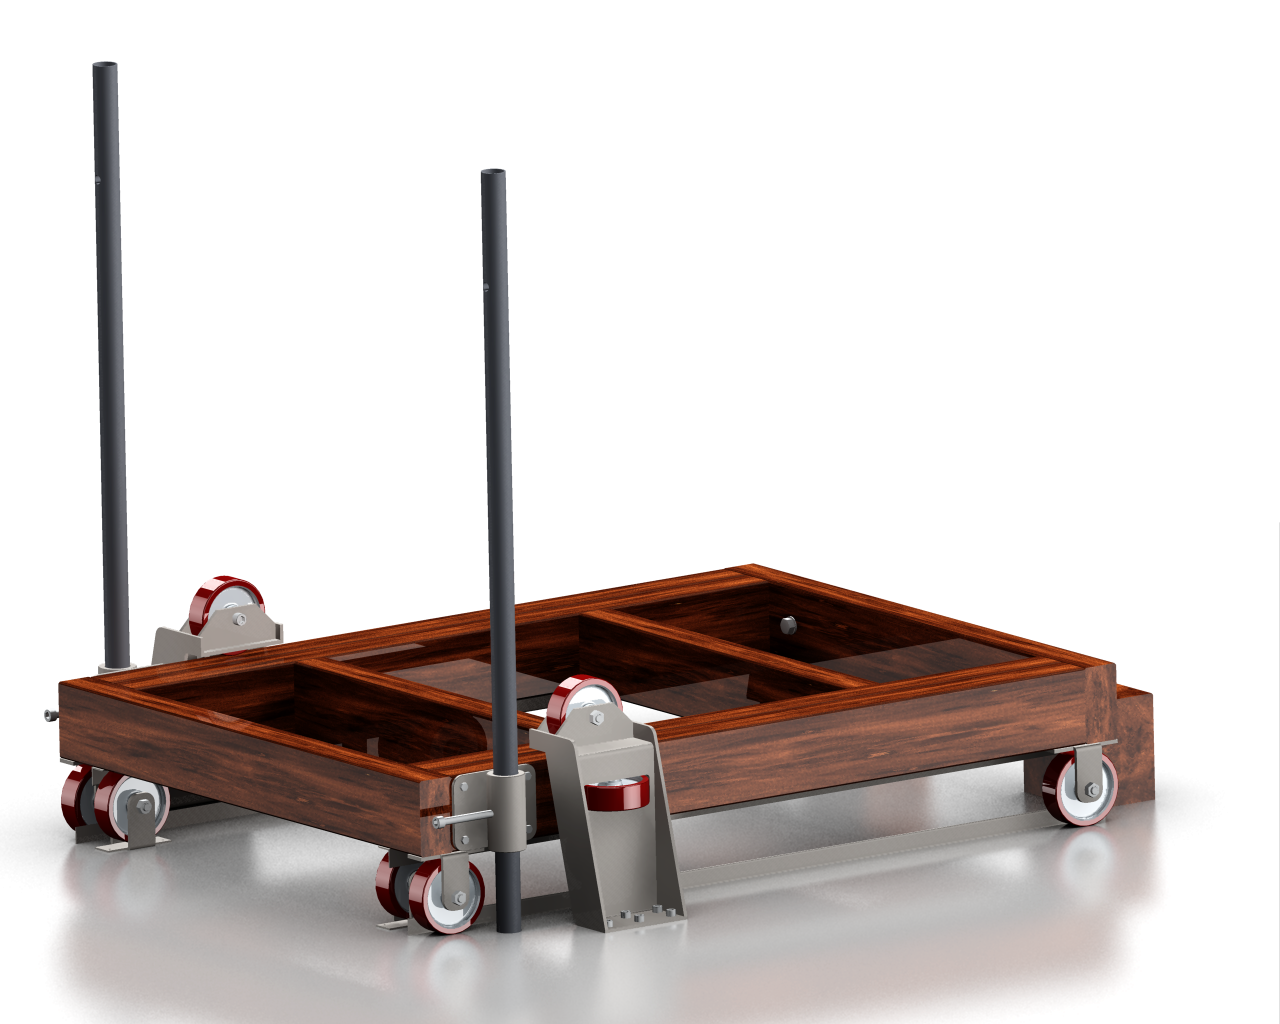
\includegraphics [width=15cm]{images/1.png}}
\caption{Sammenstilling}
\label{F1}
\end{figure}

\subsubsection{Rammen}
Den trefargede rammen er ikke modlert i full skala, dette for å gjøre det enklere å se detaljene. 
Rammen står på fire hjul. Disse hjulene hviler på gulvplanet i hengeren. Samtidig er det skrudd to hjul på selve hengerplanet, for å støtte rammen når den blir ført opp på skråplanet og videre inn i hengeren. Se Figur \ref{F1}. Selve rammen er den samme som brukt tidligere, og er som Figur \ref{F1} antyder laget av tre. På undersiden av rammen er det skrudd fast to vinkelstål som Figur \ref{F2} viser. Disse blir brukt for å lede hjulene montert på hengerplanet slik at de treffer rammen i korrekt posisjon. 
Det er også festet to vinkelstål på selve hengerplanet. Disse er, i likhet med de på rammen, ment for å lede hjulene på rammen i korrekt posisjon.
 
\begin{figure}[h!]
\centerline{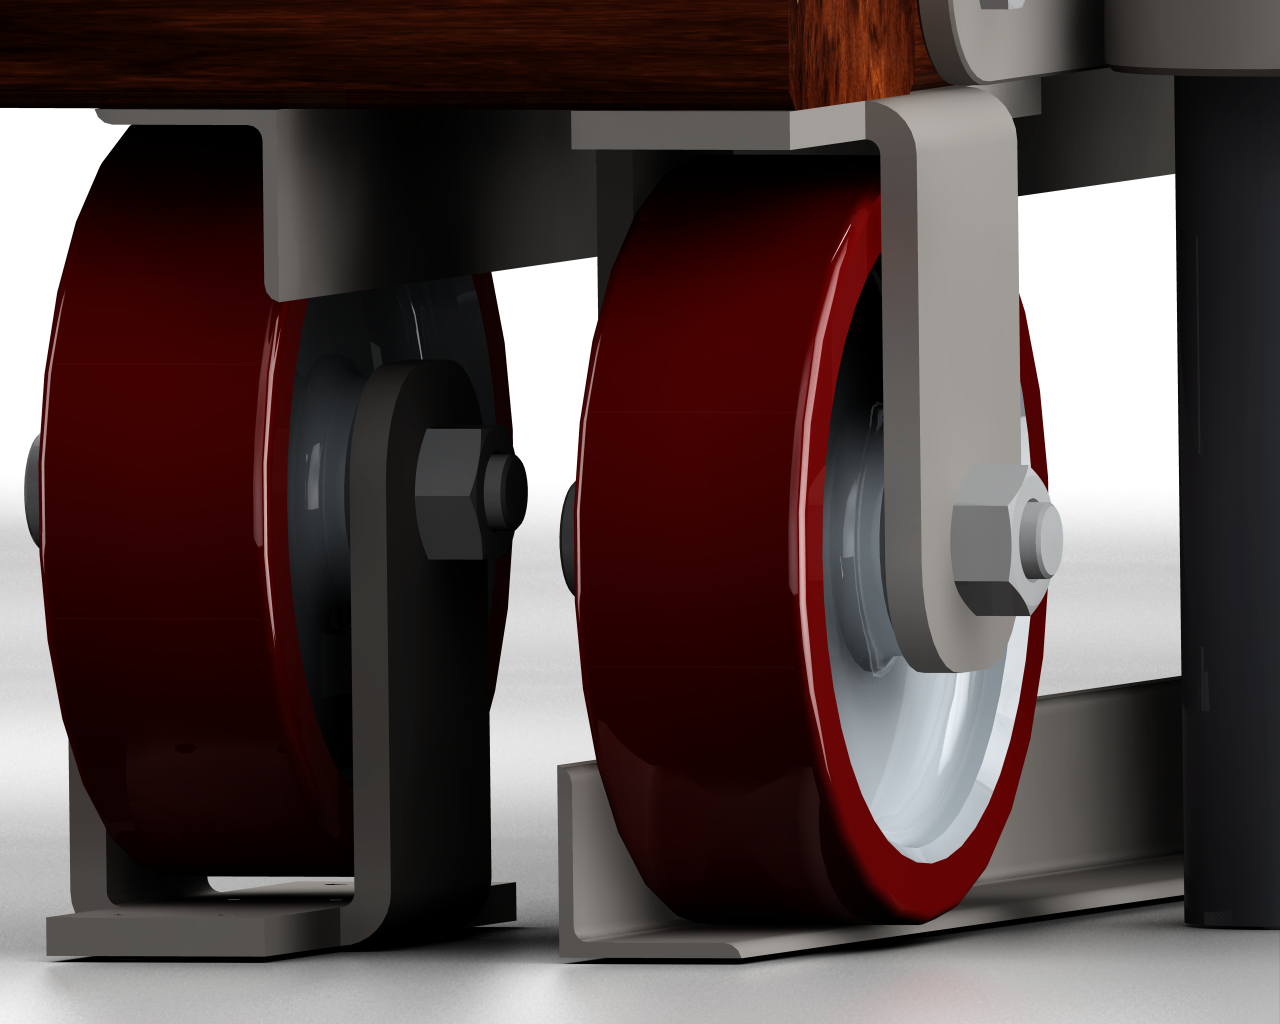
\includegraphics [width=15cm]{images/9.png}}
\caption{Vinkelstål}
\label{F2}
\end{figure}

\subsubsection{Hjulbraketter}

Hjulbrakettene er utformet sm Figur \ref{F3} viser. Disse er utformet i stålkvalitet S355J0. 
Hjulene blir festet til hjulbrakettene med M10 sylinderskruer og låsemuttere. Brakettene blir festet både til rammen og til hengerplanet ved hjelp av enkle treskruer. Hjulene er primært utsatt for trykk, svært små bøyekrefter. Dette gjør det forsvarlig å fetste disse på denne måten. Hvert hjul har en oppgitt bærekappasitet på 125 kg 

\begin{figure}[h!]
\centering   
\subfloat[Hjulbrakett Venstre]{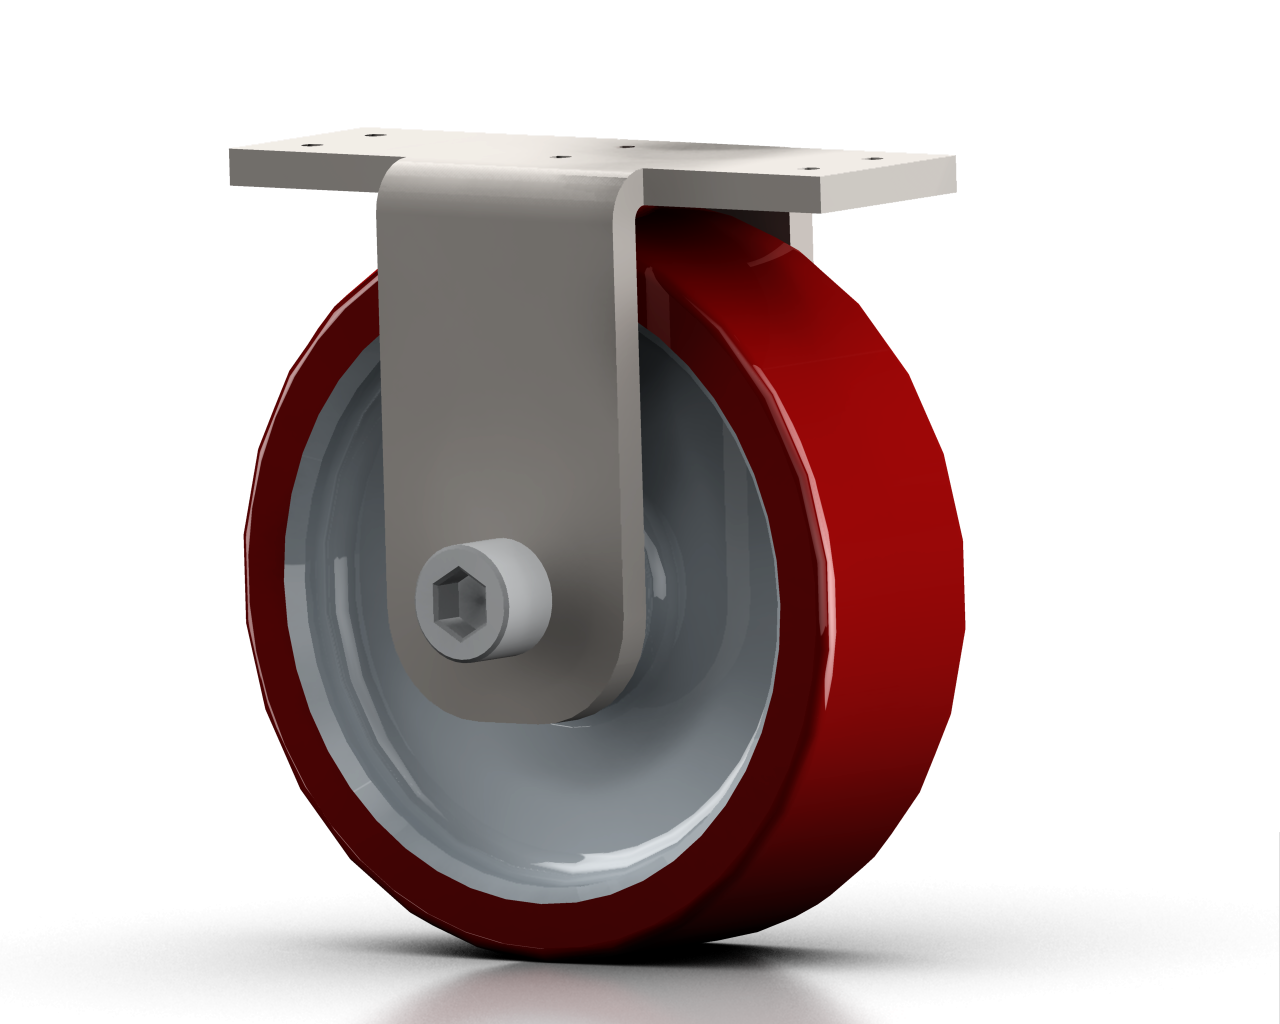
\includegraphics[width=0.5\textwidth]{images/4.png}}
\subfloat[Hjulbrakett Høyre]{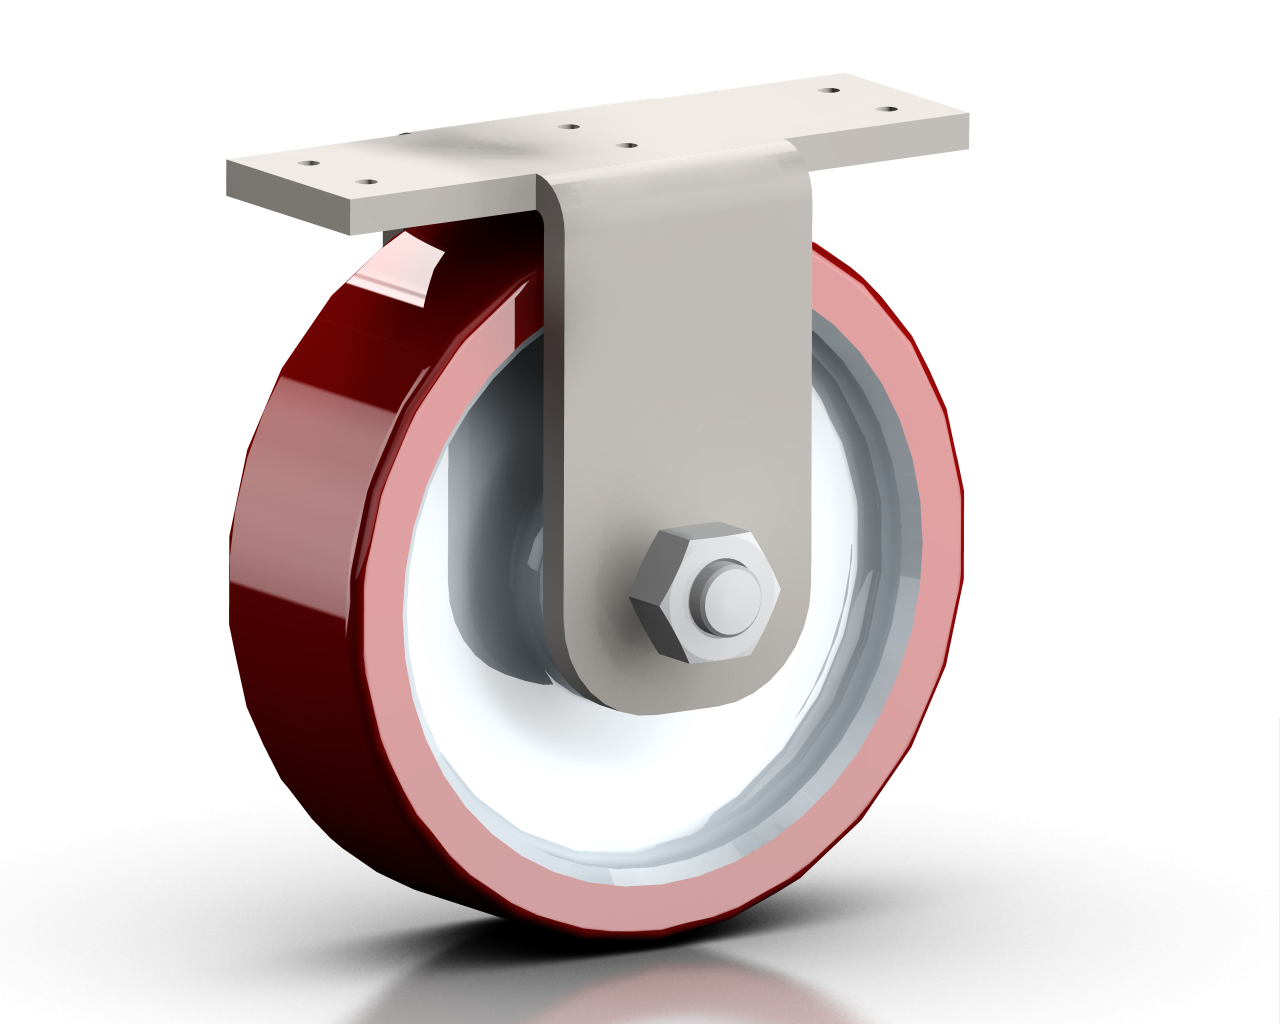
\includegraphics[width=0.5\textwidth]{images/5.png}}
\caption{Hjulbrakett}
\label{F3}
\end{figure}

\subsubsection{Støttebraketter}

Støttebralkettene skal utformes som vist i Figur \ref{F4}. Stålkvaliteten er også for disse S355J0. Platene er laserkuttet og sveist sammen med TIG på utsidene, buttsveiser, og MIG på innsidene, kilsveiser. Hjulene er laget av plastikk, med gummihjulbaner og er opplagret med kulelager. Hjulene som er benyttet er de samme som på hjulbrakettene.

\begin{figure}[h!]
\centering   
\subfloat[Støttebrakett forrfra]{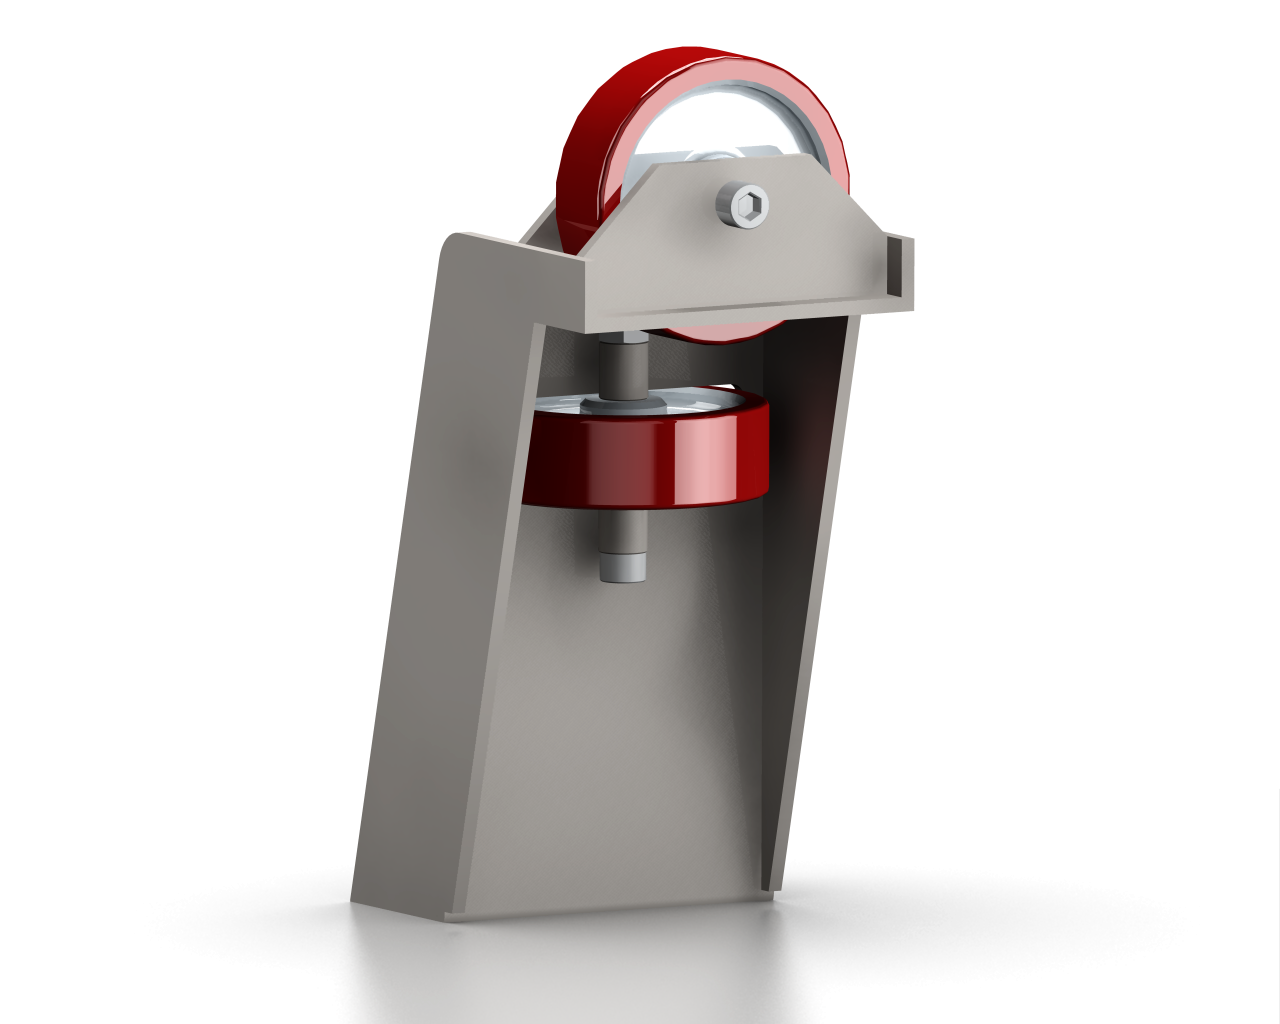
\includegraphics[width=0.5\textwidth]{images/3a.png}}
\subfloat[Støttebrakett bakfra]{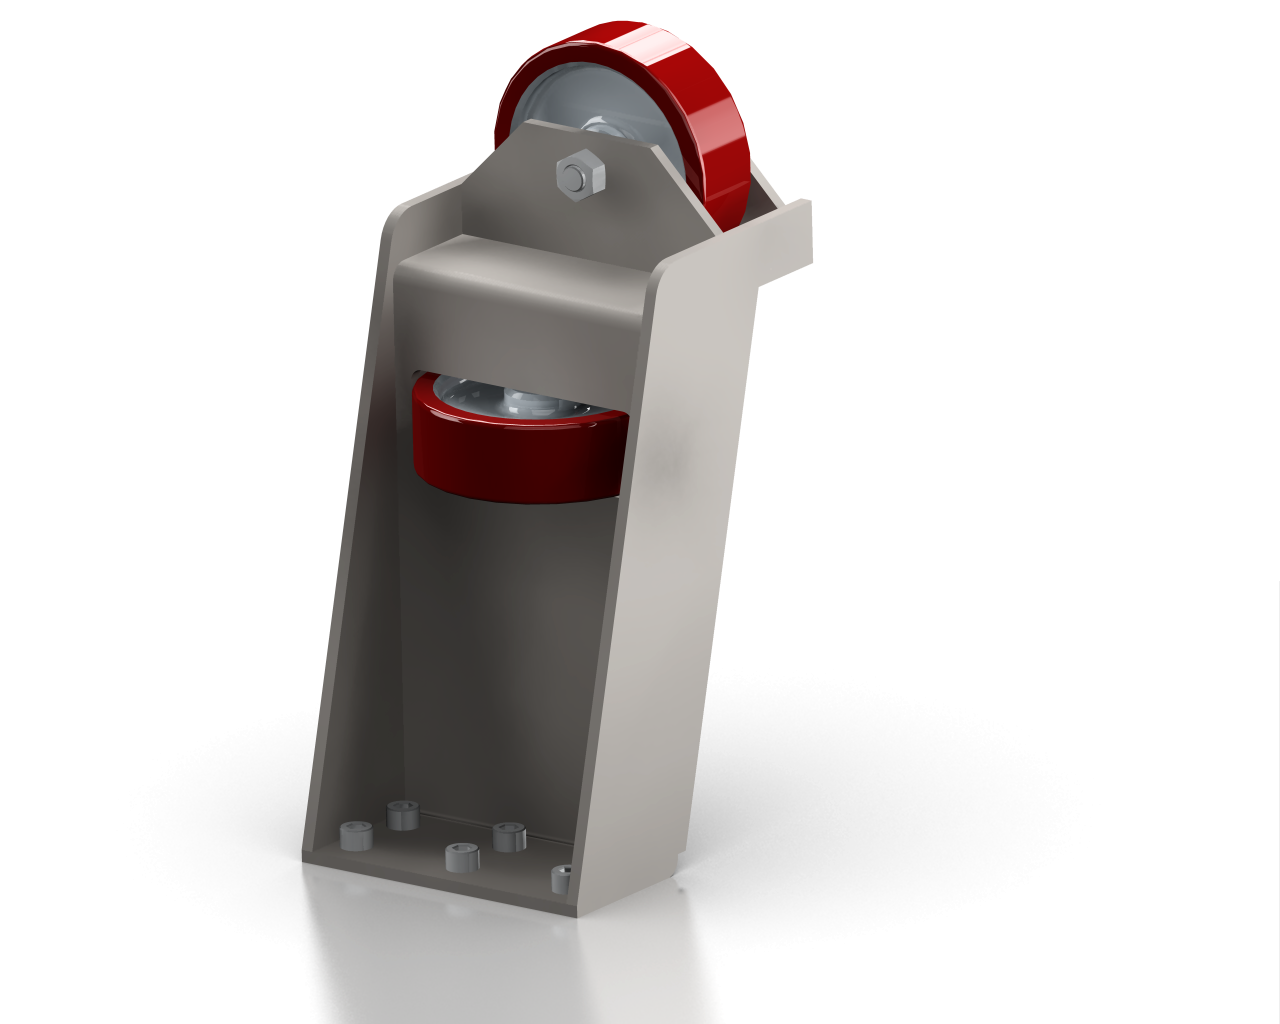
\includegraphics[width=0.5\textwidth]{images/3b.png}}
\caption{Støttebrakett}
\label{F4}
\end{figure}

Det skal benyttes M10 sylinderskruer med kvalitet 12.9 på alle hjulene. Videre skal selve braketten festet til hengeren med 6 stk, M6 syliderskruer, her også med kvalitet 12.9.    

\subsubsection{Støttebein og låsing}

Som Figur \ref{F5} viser er det designet to foringer som holder to rør. Disse rørene er ment som støtte for rammen når den blir brukt til utstilling av bilen. Altså når rammen er ute av henger mens bilen står på rammen. For mer detaljer se vedlagte arbeidstegninger og sammenstillingstegninger. Beina har både funksjon som støtte, men også som låsing i lengderetning på hengeren. Når rammen skal låses senkes beina ned på to tapper, som er boltet fast fra undersiden av hengeren. Rammen låses dermed i alle retninger. Se Figur \ref{F5}.

\begin{figure}[h!]
\centering   
\subfloat[Støtteben]{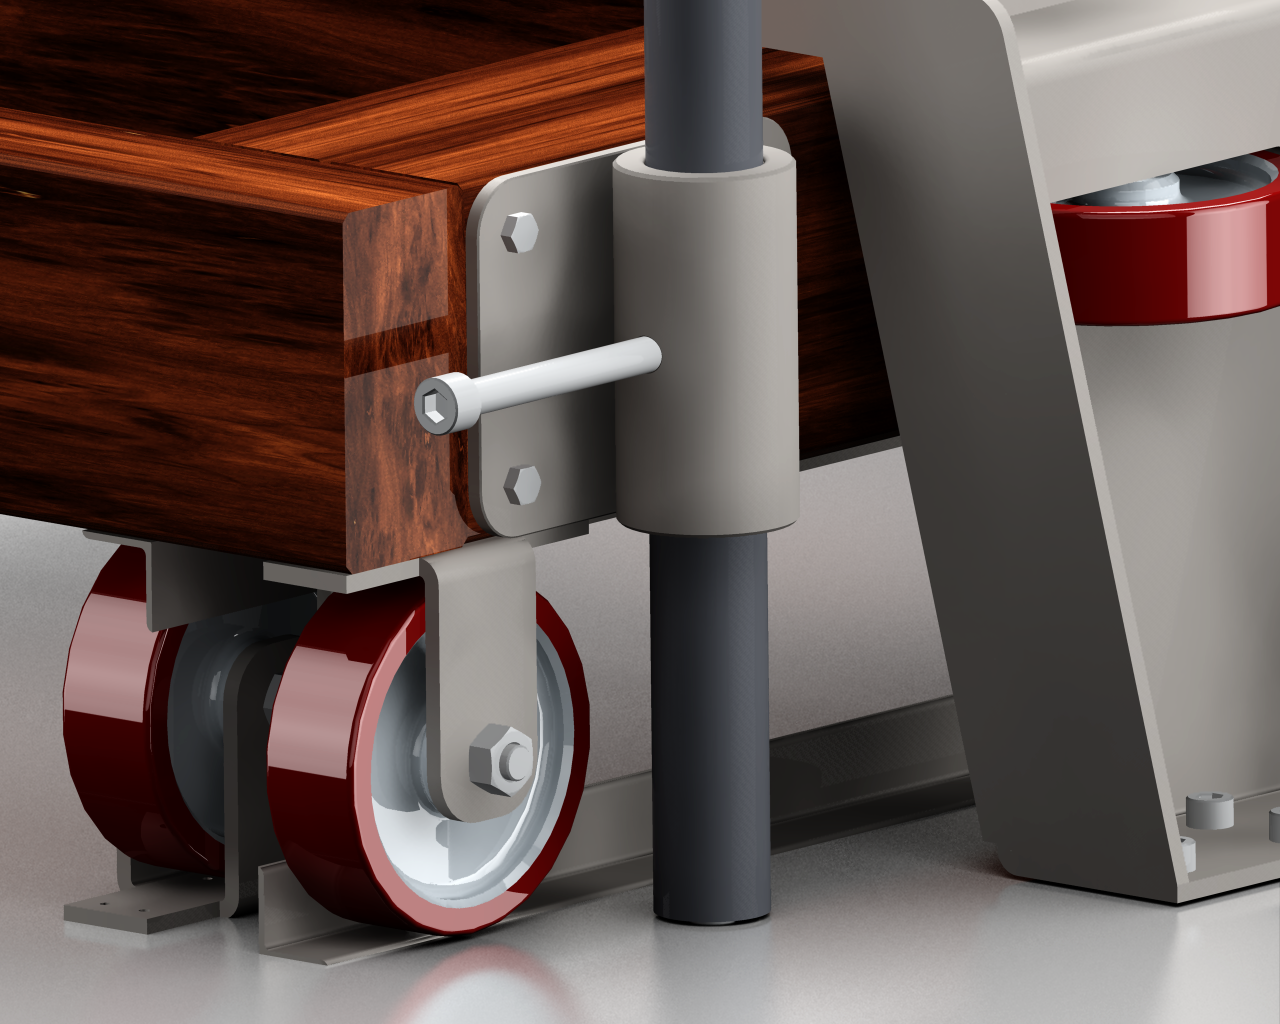
\includegraphics[width=0.4\textwidth]{images/6.png}}
\qquad
\subfloat[Låsetapp]{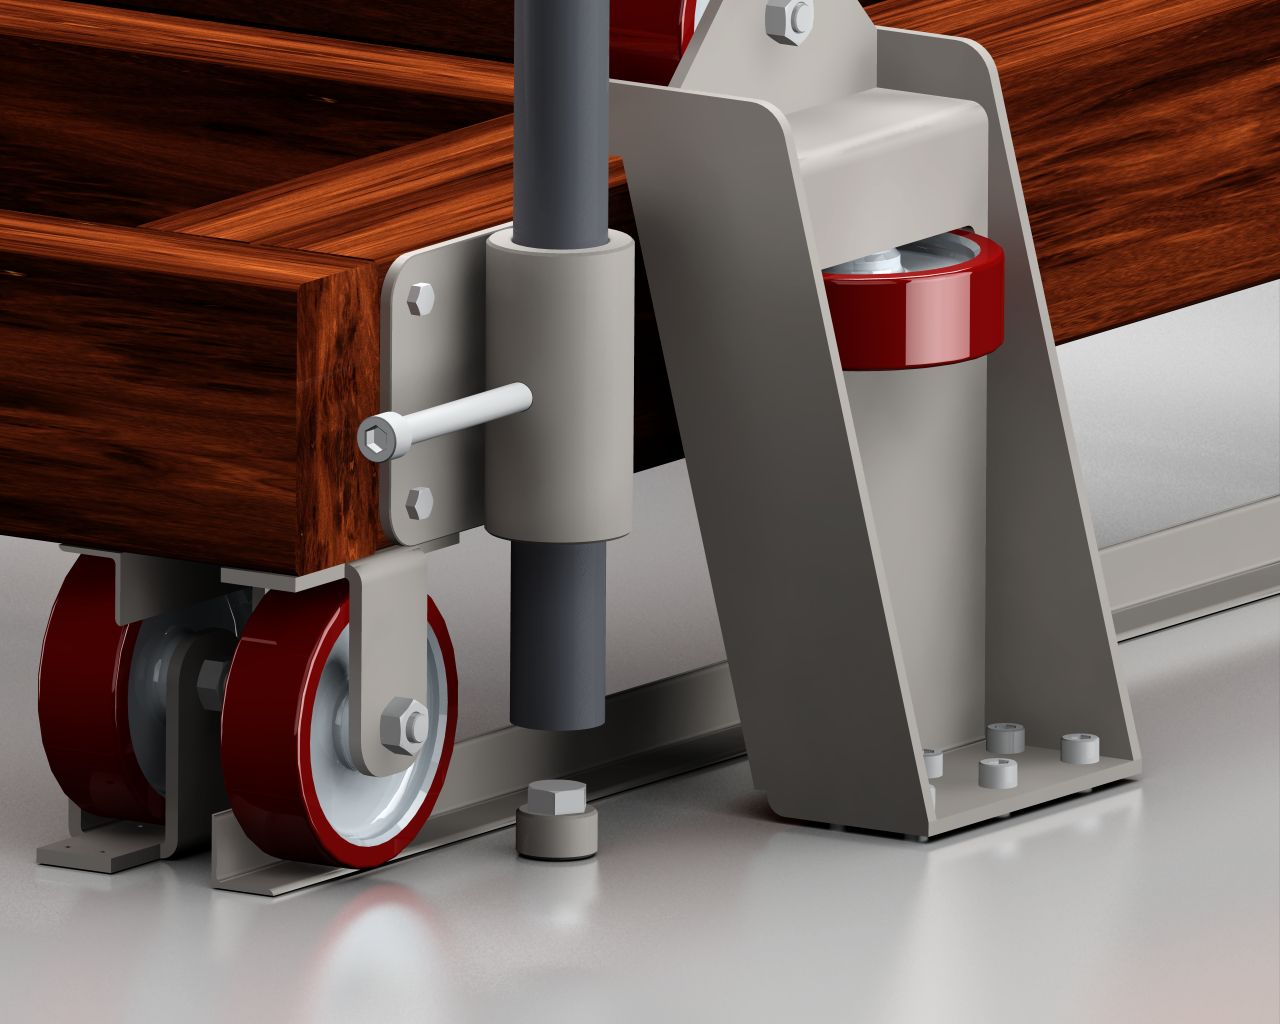
\includegraphics[width=0.4\textwidth]{images/7.png}}
\caption{Støtteben og låsing}
\label{F5}
\end{figure}

På baksiden av rammen er det festet to låsetapper. Se Figur \ref{F6}. Disse tappene har i likhet med beina funkjon som låsing. Når rammen føres inn i hengeren vil disse tappene treffe to rør som er festet til en brakett. Rammen blir slik også låst fra baksiden.  

\begin{figure}[h!]
\centerline{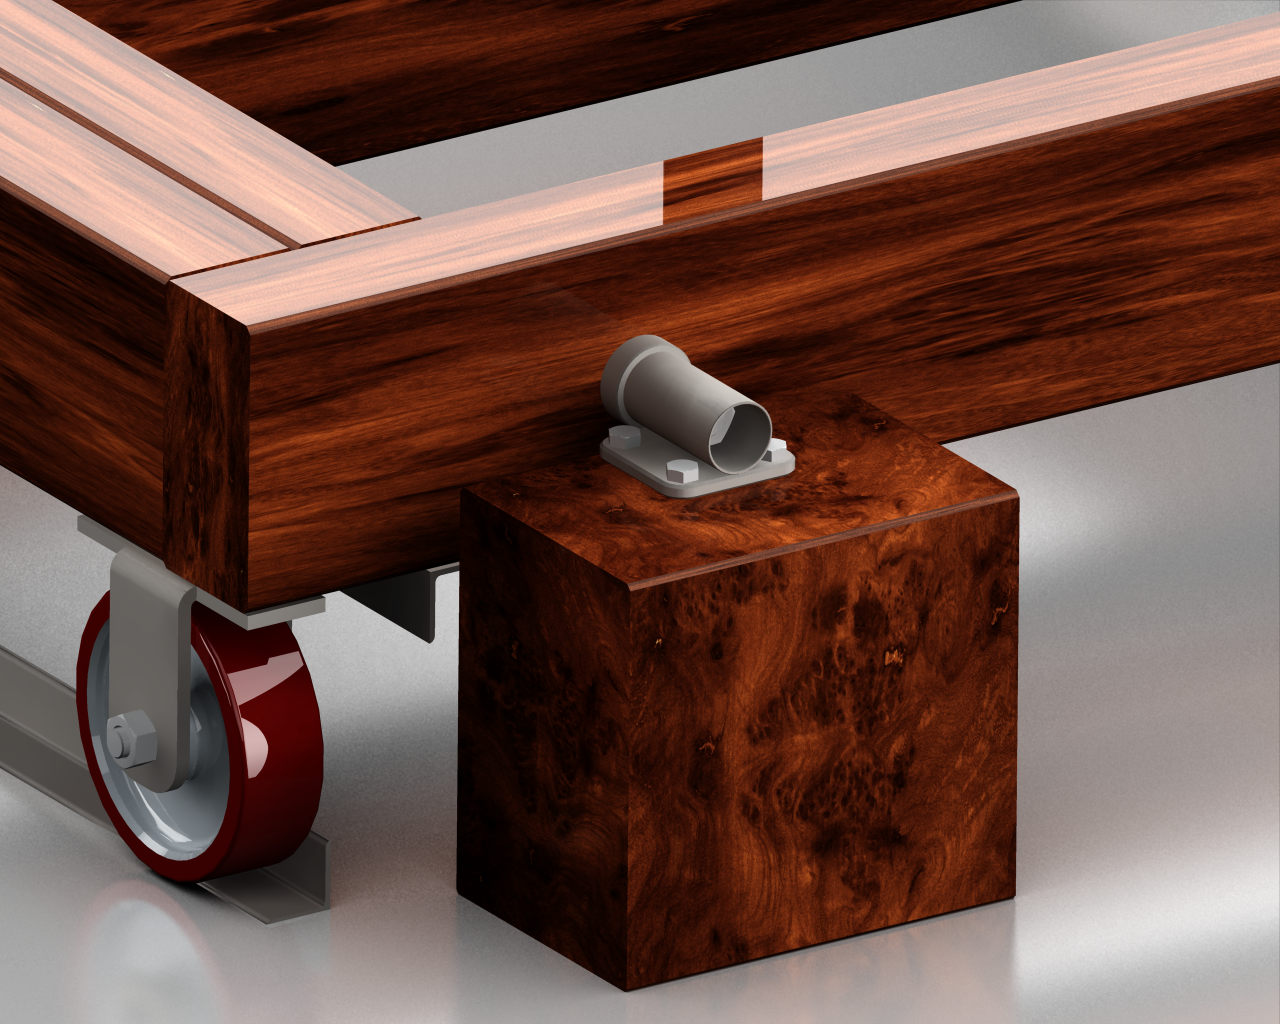
\includegraphics [width=7cm]{images/8.png}}
\caption{Låsetapper}
\label{F6}
\end{figure}
